\documentclass{beamer}

\mode<presentation>
{
  \usetheme{PaloAlto}     % Darmstadt, Madrid, Warsaw, ...
  \usecolortheme{default} % albatross, beaver, crane, ...
  \usefonttheme{default}  % serif, structurebold, ...
  \setbeamertemplate{navigation symbols}{}
  \setbeamertemplate{caption}[numbered]
} 

\usepackage[english]{babel}
\usepackage[utf8]{inputenc}
\usepackage[T1]{fontenc}
\usepackage{lmodern}
\usepackage{fontawesome5}
\usepackage{txfonts}


\title[Statistic framework of the flexible RNA]{Dimensionality reduction methods on the flexible RNA molecules}
\author{Wandrille Buchy}
\institute{ENSAI, LAAS}
\date{18.\,06.\,2026}

\begin{document}

\begin{frame}

  \titlepage
    \vfill 
  \begin{columns}[b] 
    \begin{column}{0.5\textwidth}
      \raggedright 
      
\includegraphics[height=2.4cm]{Ensai-logo.png}
    \end{column}

    \begin{column}{0.5\textwidth}
      \raggedleft 
      \raisebox{0.5cm}{
\includegraphics[height=1.3cm]{logo_LAAS.png}}
    \end{column}
  \end{columns}
  
\end{frame}

\section{Goals of the validation}

\begin{frame}{Goals}

    \begin{block}{Goal}
        ($\alpha_1,\ldots, \alpha_K$) $\in \mathbb{T}^K$, $7 \leq K \leq 12$ $\rightarrow$ \text{Two-dimensional Space}
    \end{block}

    \vskip 0.5 cm

    \begin{itemize}
        \item \textbf{Goal 1} : Evaluation of the State-of-the-Art.
        \item \textbf{Goal 2} : Study of the dependency between the angles to build another representation.
    \end{itemize}

\end{frame}

\section{State-of-the-Art}

\subsection{Dimensionality reduction}

\begin{frame}{Dimensionality reduction}

    \begin{figure}[htb]
        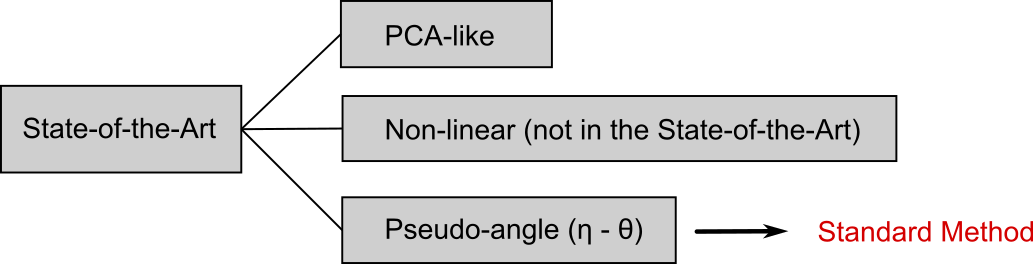
\includegraphics[width=.8\textwidth]{SOTA.png}
    \end{figure}

    \begin{figure}[htb]
        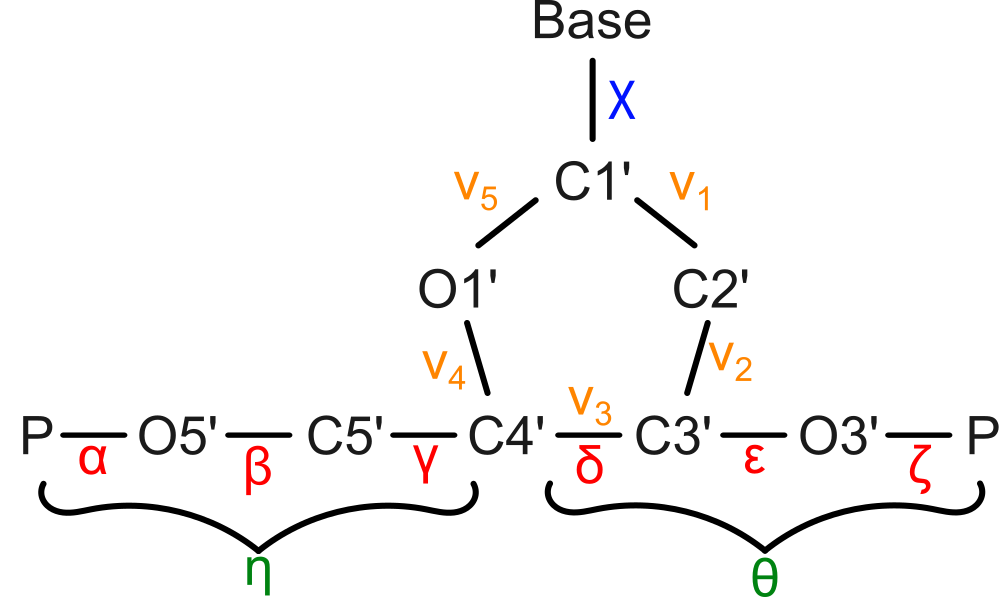
\includegraphics[width=.6\textwidth]{ARN_schema.png}
    \end{figure}

\end{frame}

\subsection{$\eta$ - $\theta$ pseudo-angles}

\begin{frame}{$\eta - \theta$ pseudo-angles}

    \begin{figure}[htb]
        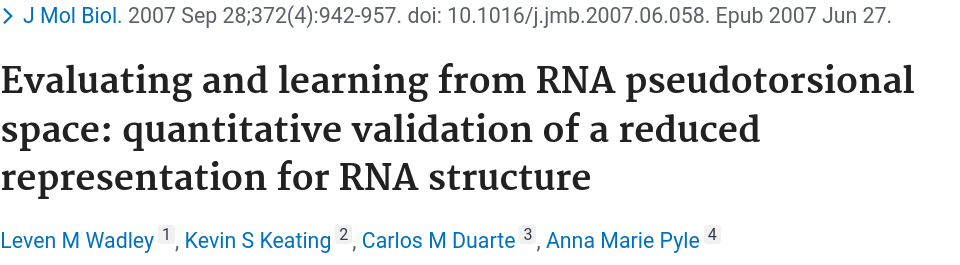
\includegraphics[width=.8\textwidth]{Evaluating - Wadley.png}
    \end{figure}

    \begin{figure}[htb]
        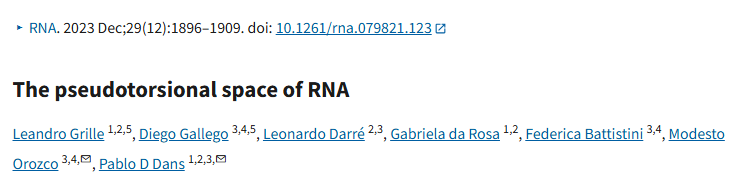
\includegraphics[width=.8\textwidth]{Pseudotorsional space of RNA.png}
    \end{figure}

    $\rightarrow$ \text{We tried to do better !}

\end{frame}

\section{Results}

\begin{frame}{Validation results}

    \begin{figure}[htb]
        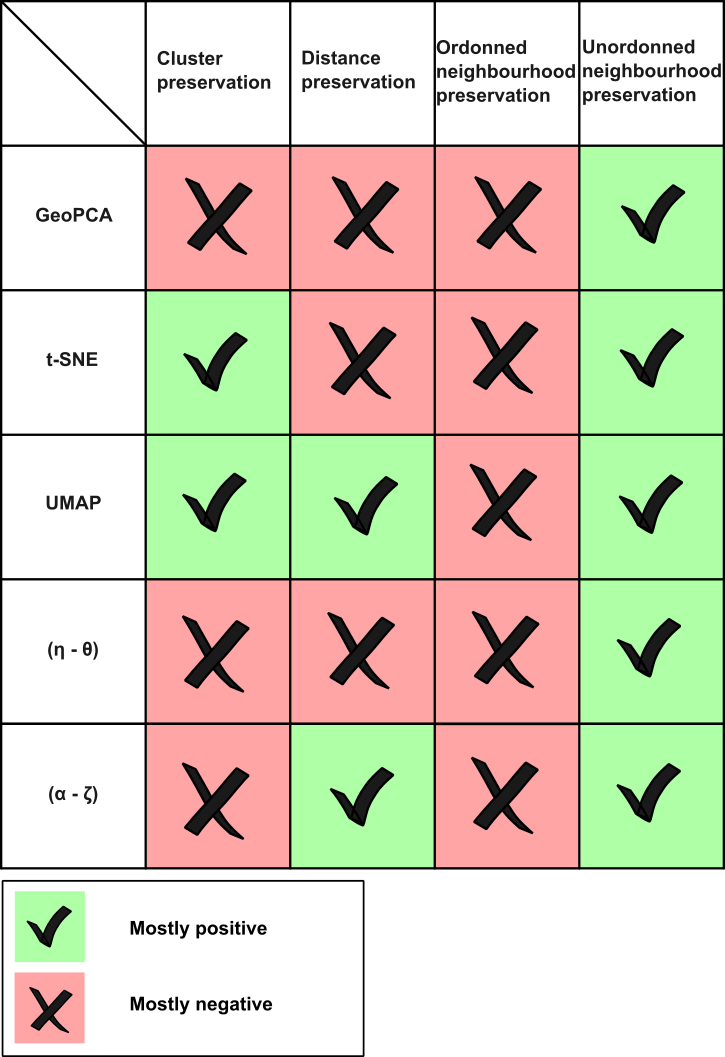
\includegraphics[width=.5\textwidth]{tab_results.png}
    \end{figure}

\end{frame}

\section{$\eta$ - $\theta$ limitations}

\begin{frame}{$\eta$ - $\theta$ limitations}
    \faExclamationTriangle \text{ 2 clusters in $\mathbb{T}^d$} $\rightarrow$ \text{1 cluster in $\mathbb{T}^2$.}

    \vskip 0.5 cm

    \begin{figure}[htb]
        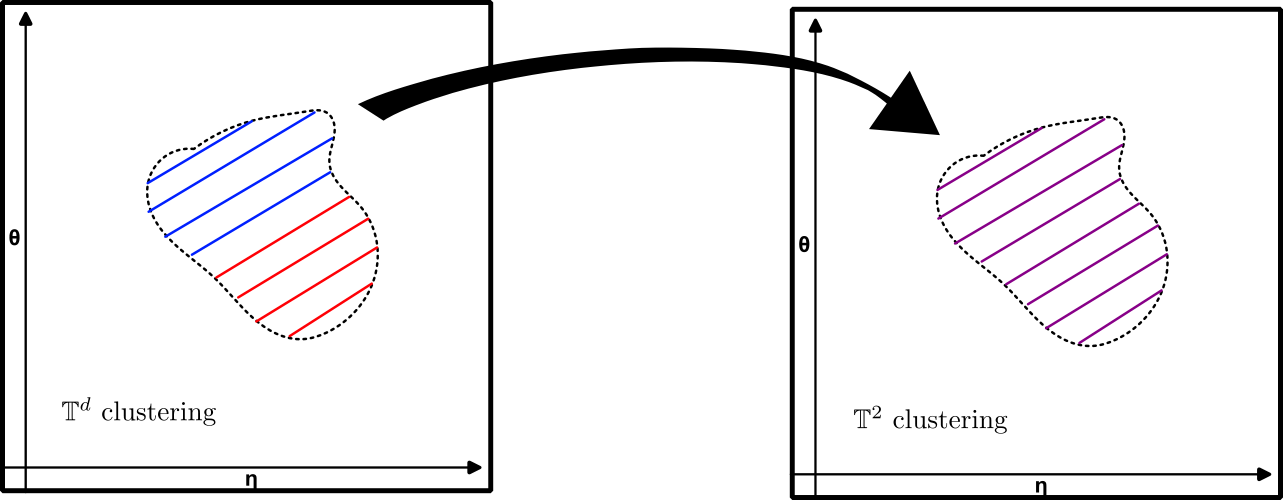
\includegraphics[width=.85\textwidth]{eta-theta_limitations.png}
    \end{figure}

    \begin{block}{Conclusion}
        \text{We lose information so we need a different method.}
    \end{block}

    \textit{Additional analysis confirm such phenomenon and its independence with the conformation.}
    
\end{frame}

\begin{frame}{$\eta$ - $\theta$ limitations}

    \begin{figure}[htb]
        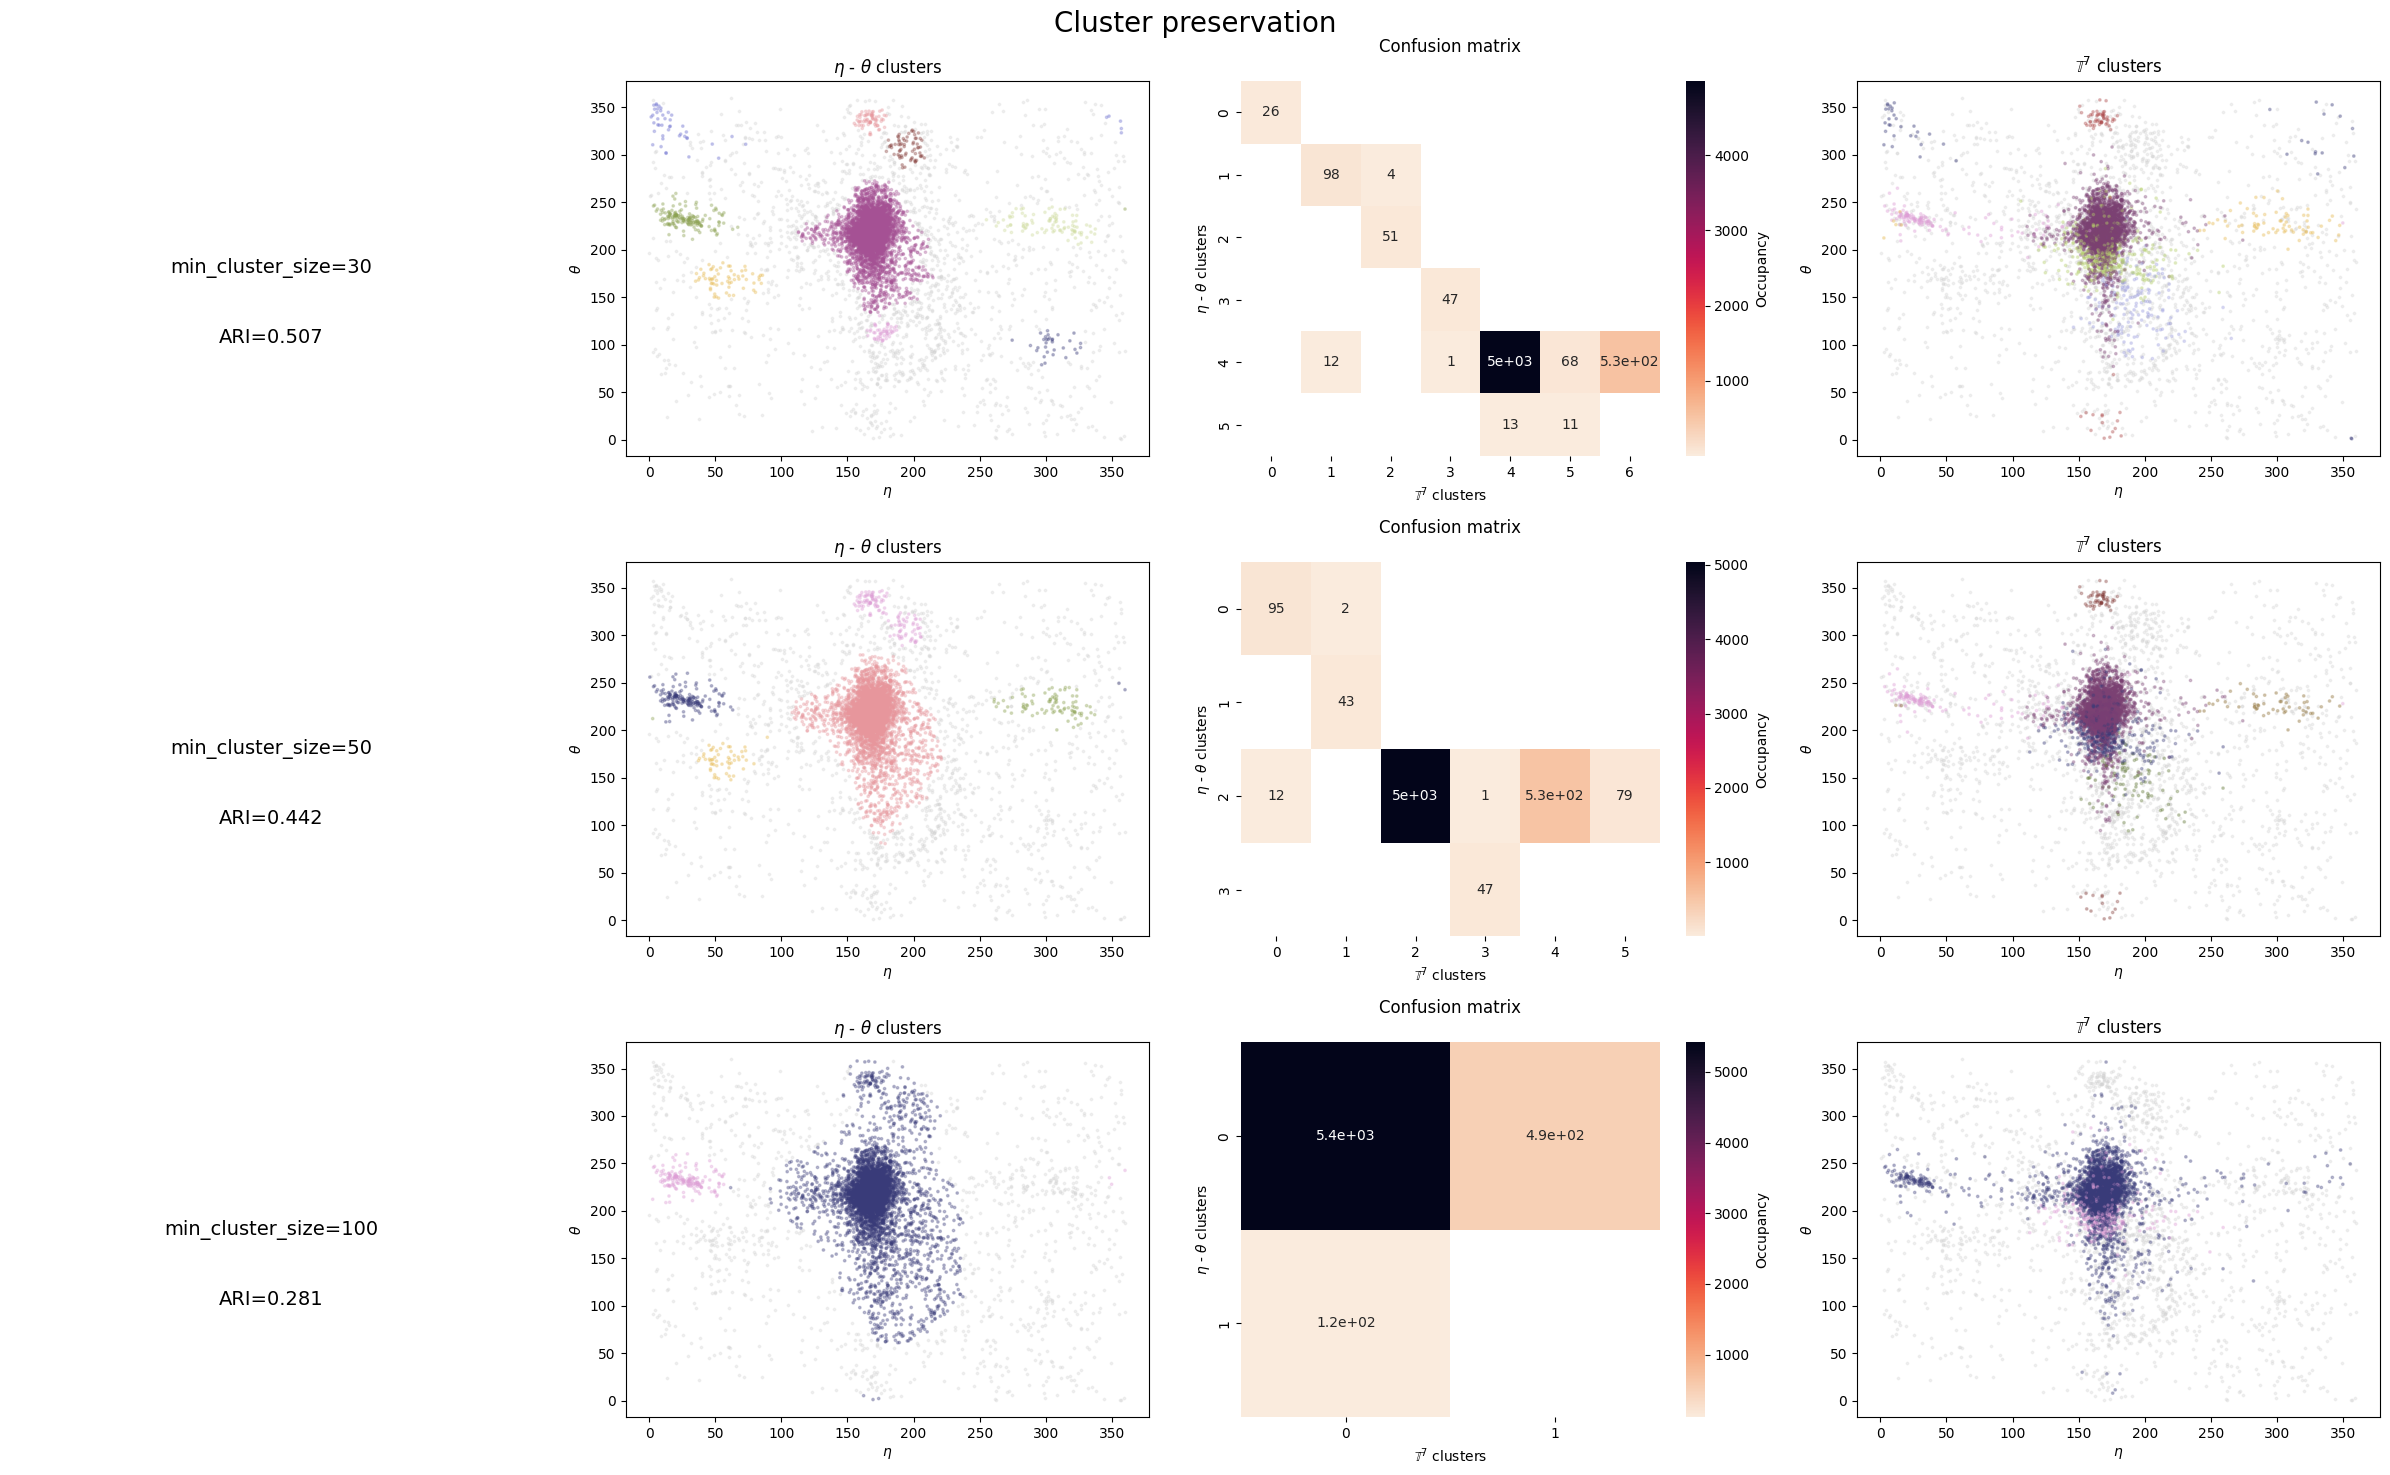
\includegraphics[width=.88\textwidth]{HDBSCAN_pseuo_T7_compars.png}
    \end{figure}

    $\rightarrow$ We got two clusters in the dense area in $\mathbb{T}^7$ but only one for the $\eta$ - $\theta$ method.
    
\end{frame}

\section{Goal of the dependency}

\subsection{Goal}

\begin{frame}{Goal}

    \begin{block}{Goal}
        For each pair of angles ($\alpha$, $\beta$), we want to test : \\
        \begin{center}
            $H_0$ : $\alpha\Perp\beta$
        \end{center}
    \end{block}

    \vskip 0.3 cm

    \begin{figure}[htb]
        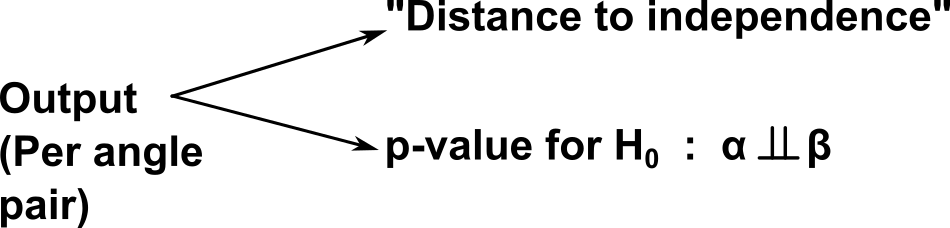
\includegraphics[width=.75\textwidth]{Output_test_dependance.png}
    \end{figure}

    {
    \setbeamercolor{block title}{bg=gray!70, fg=white}
    \setbeamercolor{block body}{bg=gray!15}
    
    \begin{block}{Remark}
        Classical test methods are not well-suited for $\mathbb{S}^1$ so we used an Optimal Transport based method.
    \end{block}
    }
    
\end{frame}

\subsection{Exemple of a representation}

\begin{frame}{Exemple of a representation}

    \begin{figure}[htb]
        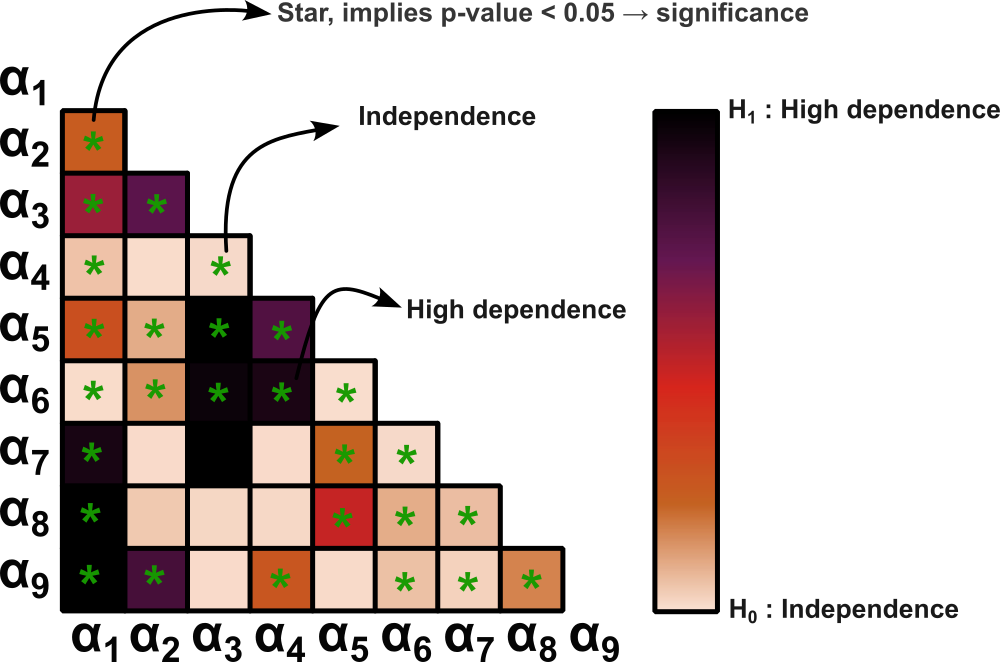
\includegraphics[width=.75\textwidth]{exemple_matrix.png}
    \end{figure}
    
\end{frame}

\section{Results}

\begin{frame}{Results of the tests}

    \begin{figure}[htb]
        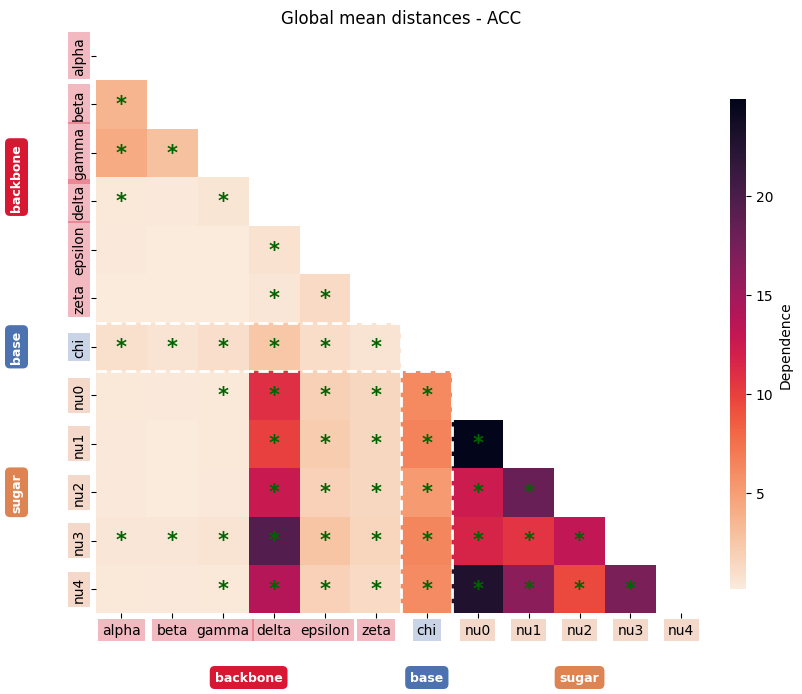
\includegraphics[width=.75\textwidth]{Matrix_Wasserstein_distance_ACC.png}
    \end{figure}
    
\end{frame}

\section{Results}

\begin{frame}{Results of the tests}

    \begin{figure}[htb]
        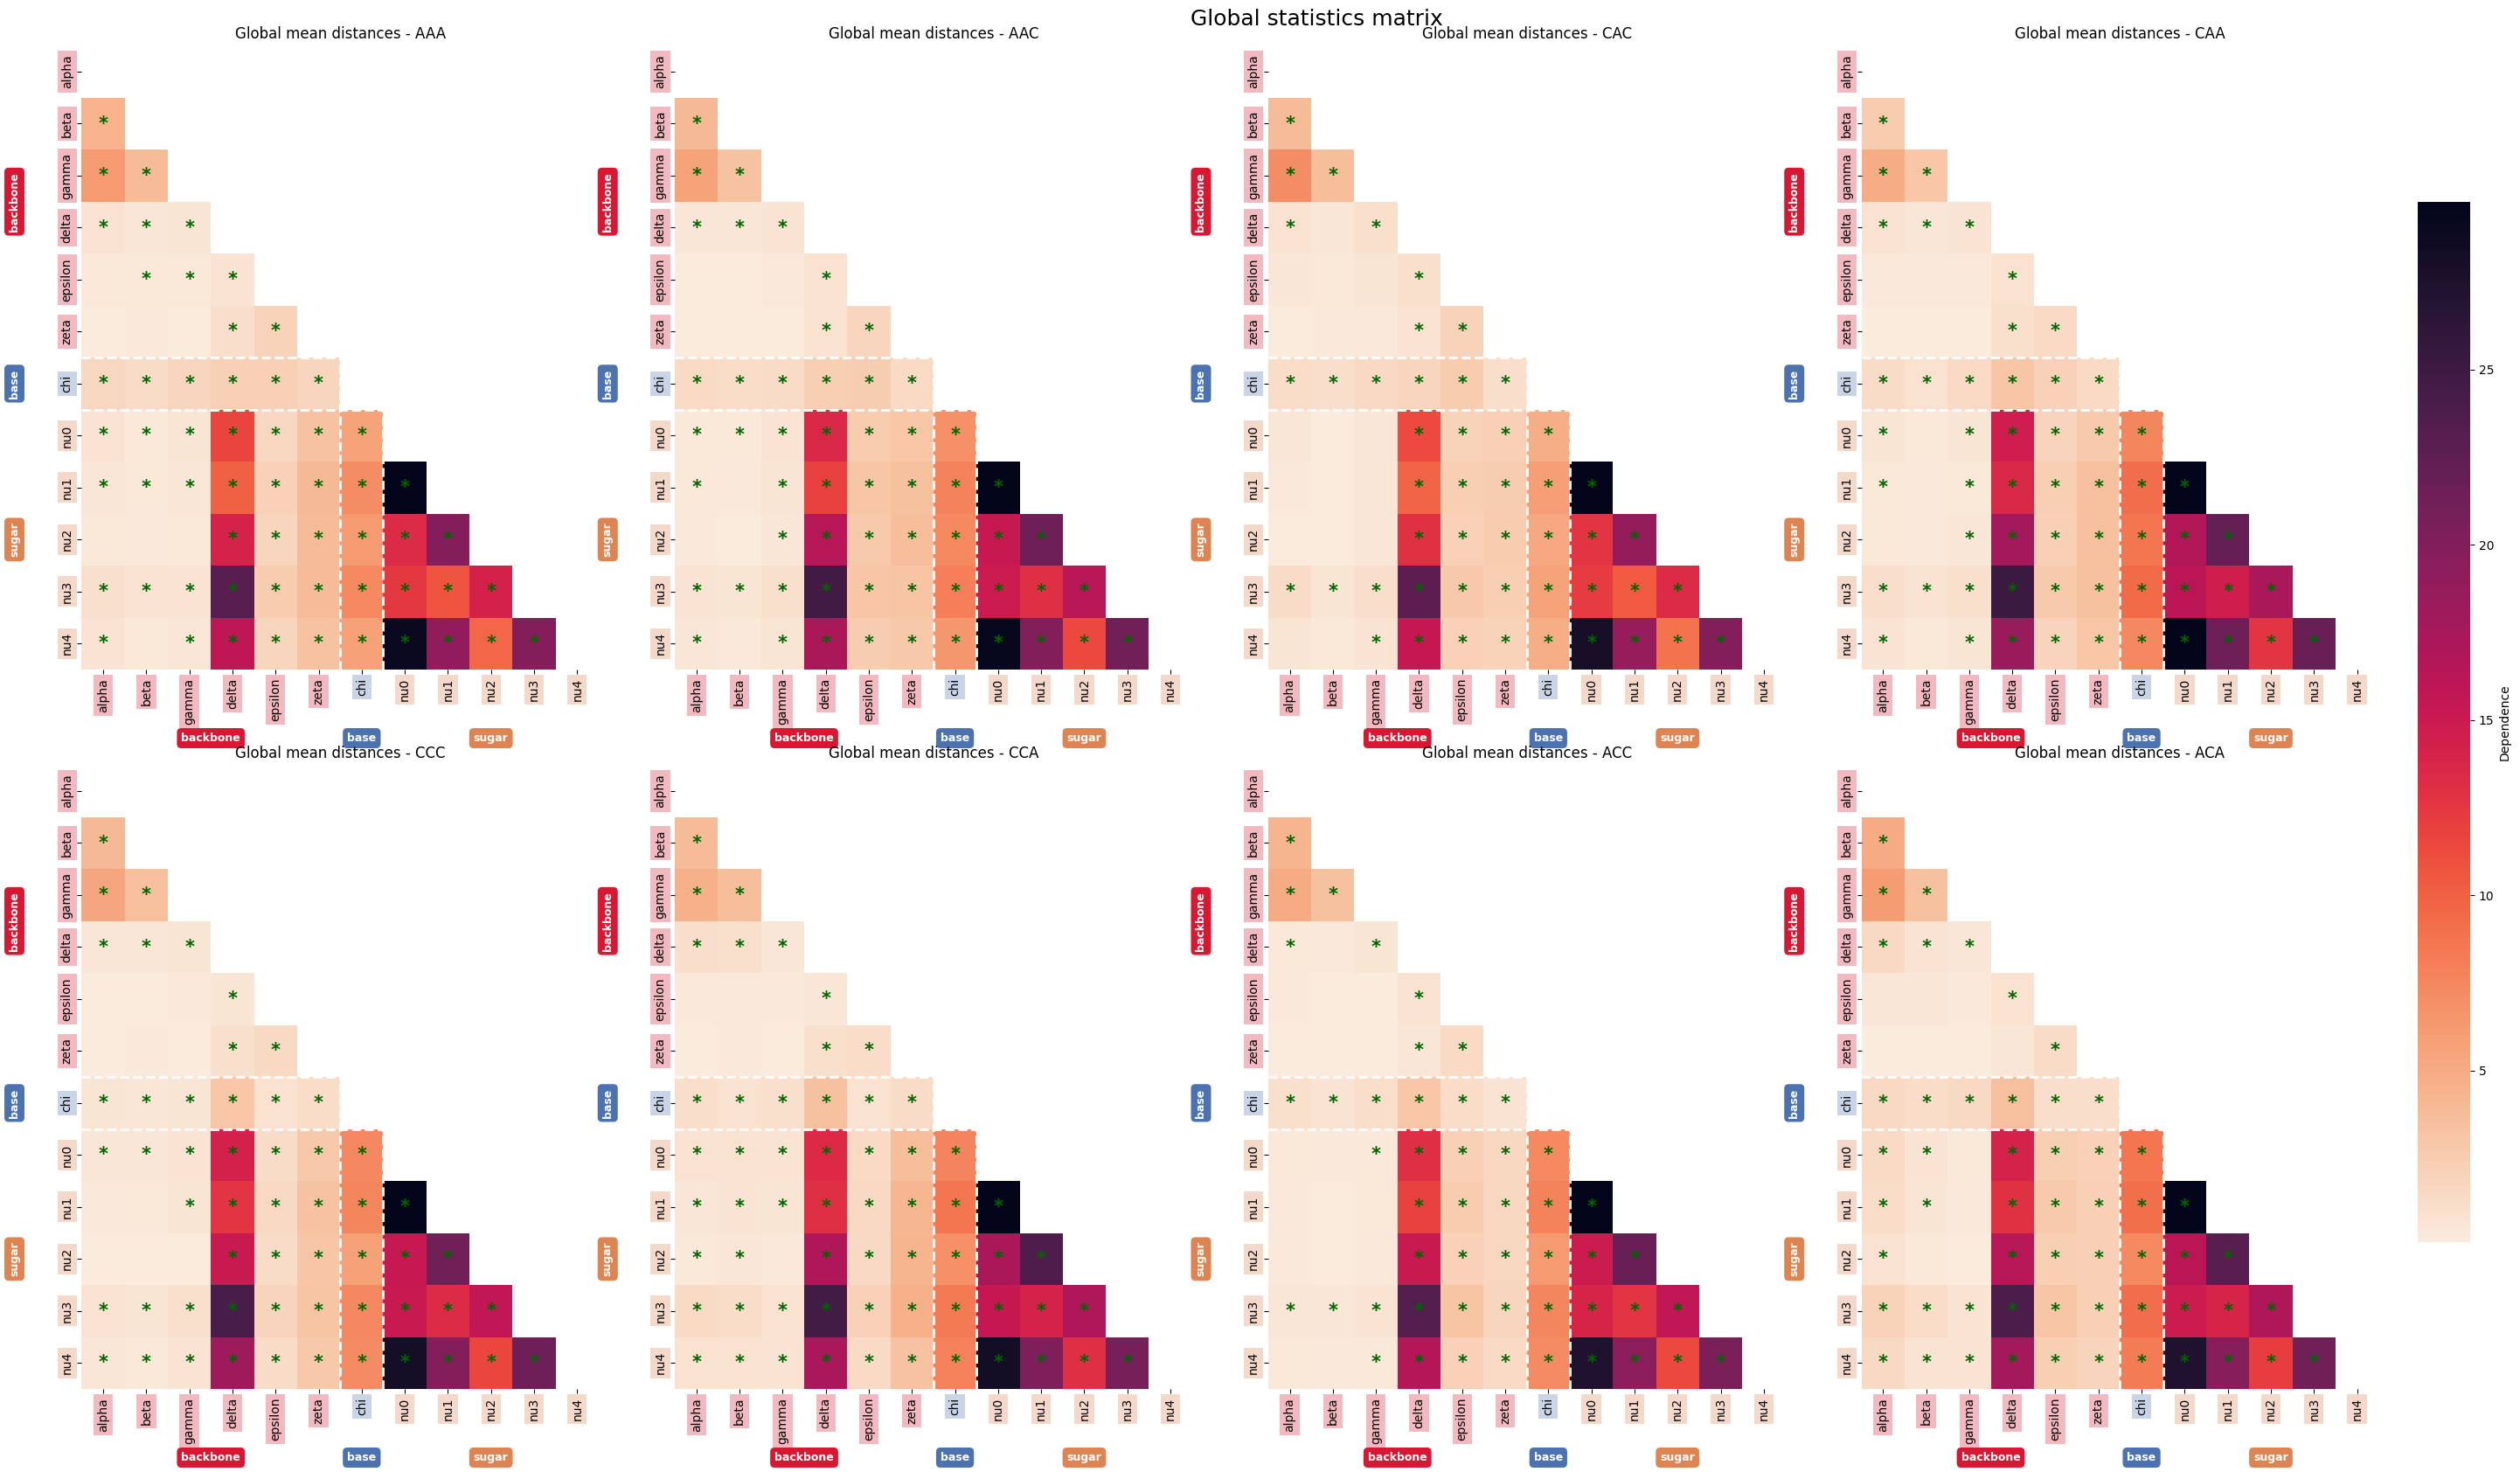
\includegraphics[width=1\textwidth]{Full_Matrix_Wasserstein_distance_ACC.png}
    \end{figure}
    
\end{frame}

\section{Next steps}

\begin{frame}{Next steps}

    \begin{itemize}
        \item Study of the independence between groups of angles.
        \item Proposition of a new pseudo-angle approach with the dependency found.
    \end{itemize}
    
\end{frame}

\end{document}
